\phantomsection
\addcontentsline{toc}{chapter}{Appendices}

% The \appendix command resets the chapter counter, and changes the chapter numbering scheme to capital letters.
%\chapter{Appendices}
\appendix
\chapter{Viewing Profiling Results}
\label{appendixlabel1}
All profiling results shown in this thesis are saved in the Git repository located \href{https://github.com/SeanBrayUCL/contur_thesis}{here}. The repository contain a Read.Me file which should make the navigation of the profiling results clear. 

To briefly summarise, the \texttt{profiles} folder in the repository contains all the profiles, its contents are shown in figure \ref{fig:profiles_folder} below. The \texttt{starting\_point} folder is the initial profile before optimisation, it contains a \say{prof} file which can be read by \textbf{Snakeviz} to create the browser interface discuss in section \ref{chapterlabel3}, additionally the folder also contain a png file which is the dot plot produced \textbf{gprof2dot} and discussed further in section \ref{chapterlabel3}.

\begin{figure}[H]
\centering
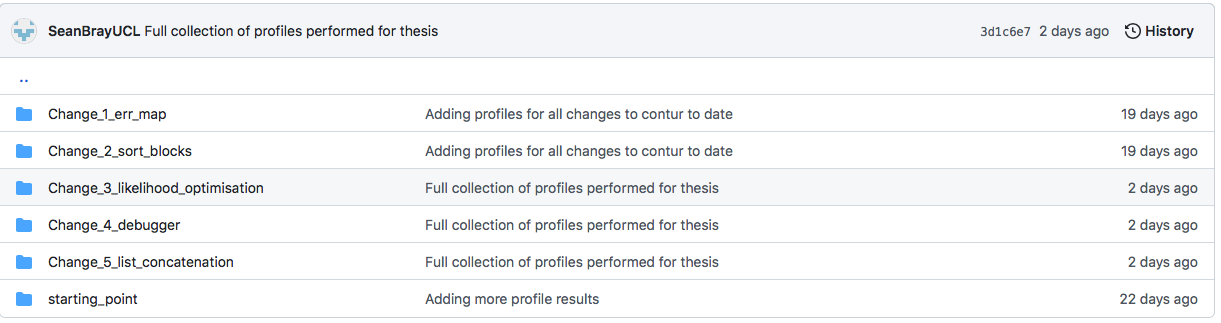
\includegraphics[scale=0.3]{plots/profiles_folder.png}
\caption{Profiles Folder}
\label{fig:profiles_folder}
\end{figure}

Each of the subsequent numbered folders are structured the same as the \texttt{starting\_point} folder. They each contain an updated profile of \textbf{Contur} after an optimisation change has been made. The optimisation changes accumulate across the folders, so the profile in folder \texttt{Change\_5\_list\_concatenation} contains all the optimisation changes, so can be taken as the complete post optimisation \textbf{Contur} profile.

\chapter{Viewing Code Written For Project}
All code written for this project, with one exception, can be found in the main \textbf{Contur} repository\cite{contur_main}. Links to specific commits made by this author can be found throughout this thesis, the approach taken has been to include a footnote with a link to the specific commits when discussing code changes in the thesis. A quick overview of code contributions to the main repository by this author can also be seen via the contributors page of the main \textbf{Contur} repository\cite{contur_main}.

